\chapter{Introduction}
\label{ch:intro}

\section{Motivation}
Stress is not directly observable. A student or engineer meets it as a tensor with six independent components, and the usual textbook solutions are closed-form results for idealised geometries: a beam, a shaft, a thin cylinder. The formulas hide the assumptions that make them valid, and the most instructive situations, such as a load on only part of a surface, have no simple closed form. An interactive tool that applies the same equations to arbitrary inputs, and states its assumptions, closes both gaps.

\section{Objectives}
The project has four objectives:
\begin{enumerate}[nosep]
\item to compute and display the stress, strain and deformation inside a solid body loaded over a user-defined patch of its surface (the \emph{3D stress field});
\item to provide analytical simulators for nine canonical problems, each reporting the governing equations beside its result (the \emph{simulators});
\item to provide a general numerical method, the finite element method, against which the analytical results can be compared (the \emph{FEM tab});
\item to verify every component against independent closed-form results, limiting cases and invariants, so that the displayed numbers can be trusted.
\end{enumerate}

\section{Scope and assumptions}
All models are \textbf{linear elastic} with \textbf{small strain}, so the principle of superposition holds and stress is proportional to load. The 3D stress field treats the body as an elastic half-space, which is exact for a body much larger than the loaded area and approximate otherwise; the finite element block (Chapter~\ref{ch:fem}) measures that approximation. Plasticity, large rotation, contact, dynamics and damage are outside the scope.

\section{Organisation of this report}
Chapter~\ref{ch:system} describes the software, its conventions and its architecture. Chapters~\ref{ch:stress}--\ref{ch:section} present the theory and implementation of the stress-at-a-point tools and the 3D field. Chapter~\ref{ch:sims} treats the nine simulators and Chapter~\ref{ch:fem} the finite element method. Chapter~\ref{ch:verify} verifies the code against independent solutions, Chapter~\ref{ch:results} shows the software in use with worked examples, and Chapter~\ref{ch:discuss} discusses limitations and concludes. The appendices cover extending the software, an index from principle to function, and the interfaces. Each theory chapter gives the \textbf{theory} first, then the \textbf{implementation} (source excerpts with line numbers).

\chapter{System overview}
\label{ch:system}
Shape Analytics is a browser application served by a small Python server. It has four groups of tools: the \textbf{3D stress field} (with section analytics), nine \textbf{analytical simulators}, and a \textbf{finite element tab}. Figure~\ref{fig:ui-field} shows the interface.

\begin{figure}[t]
\centering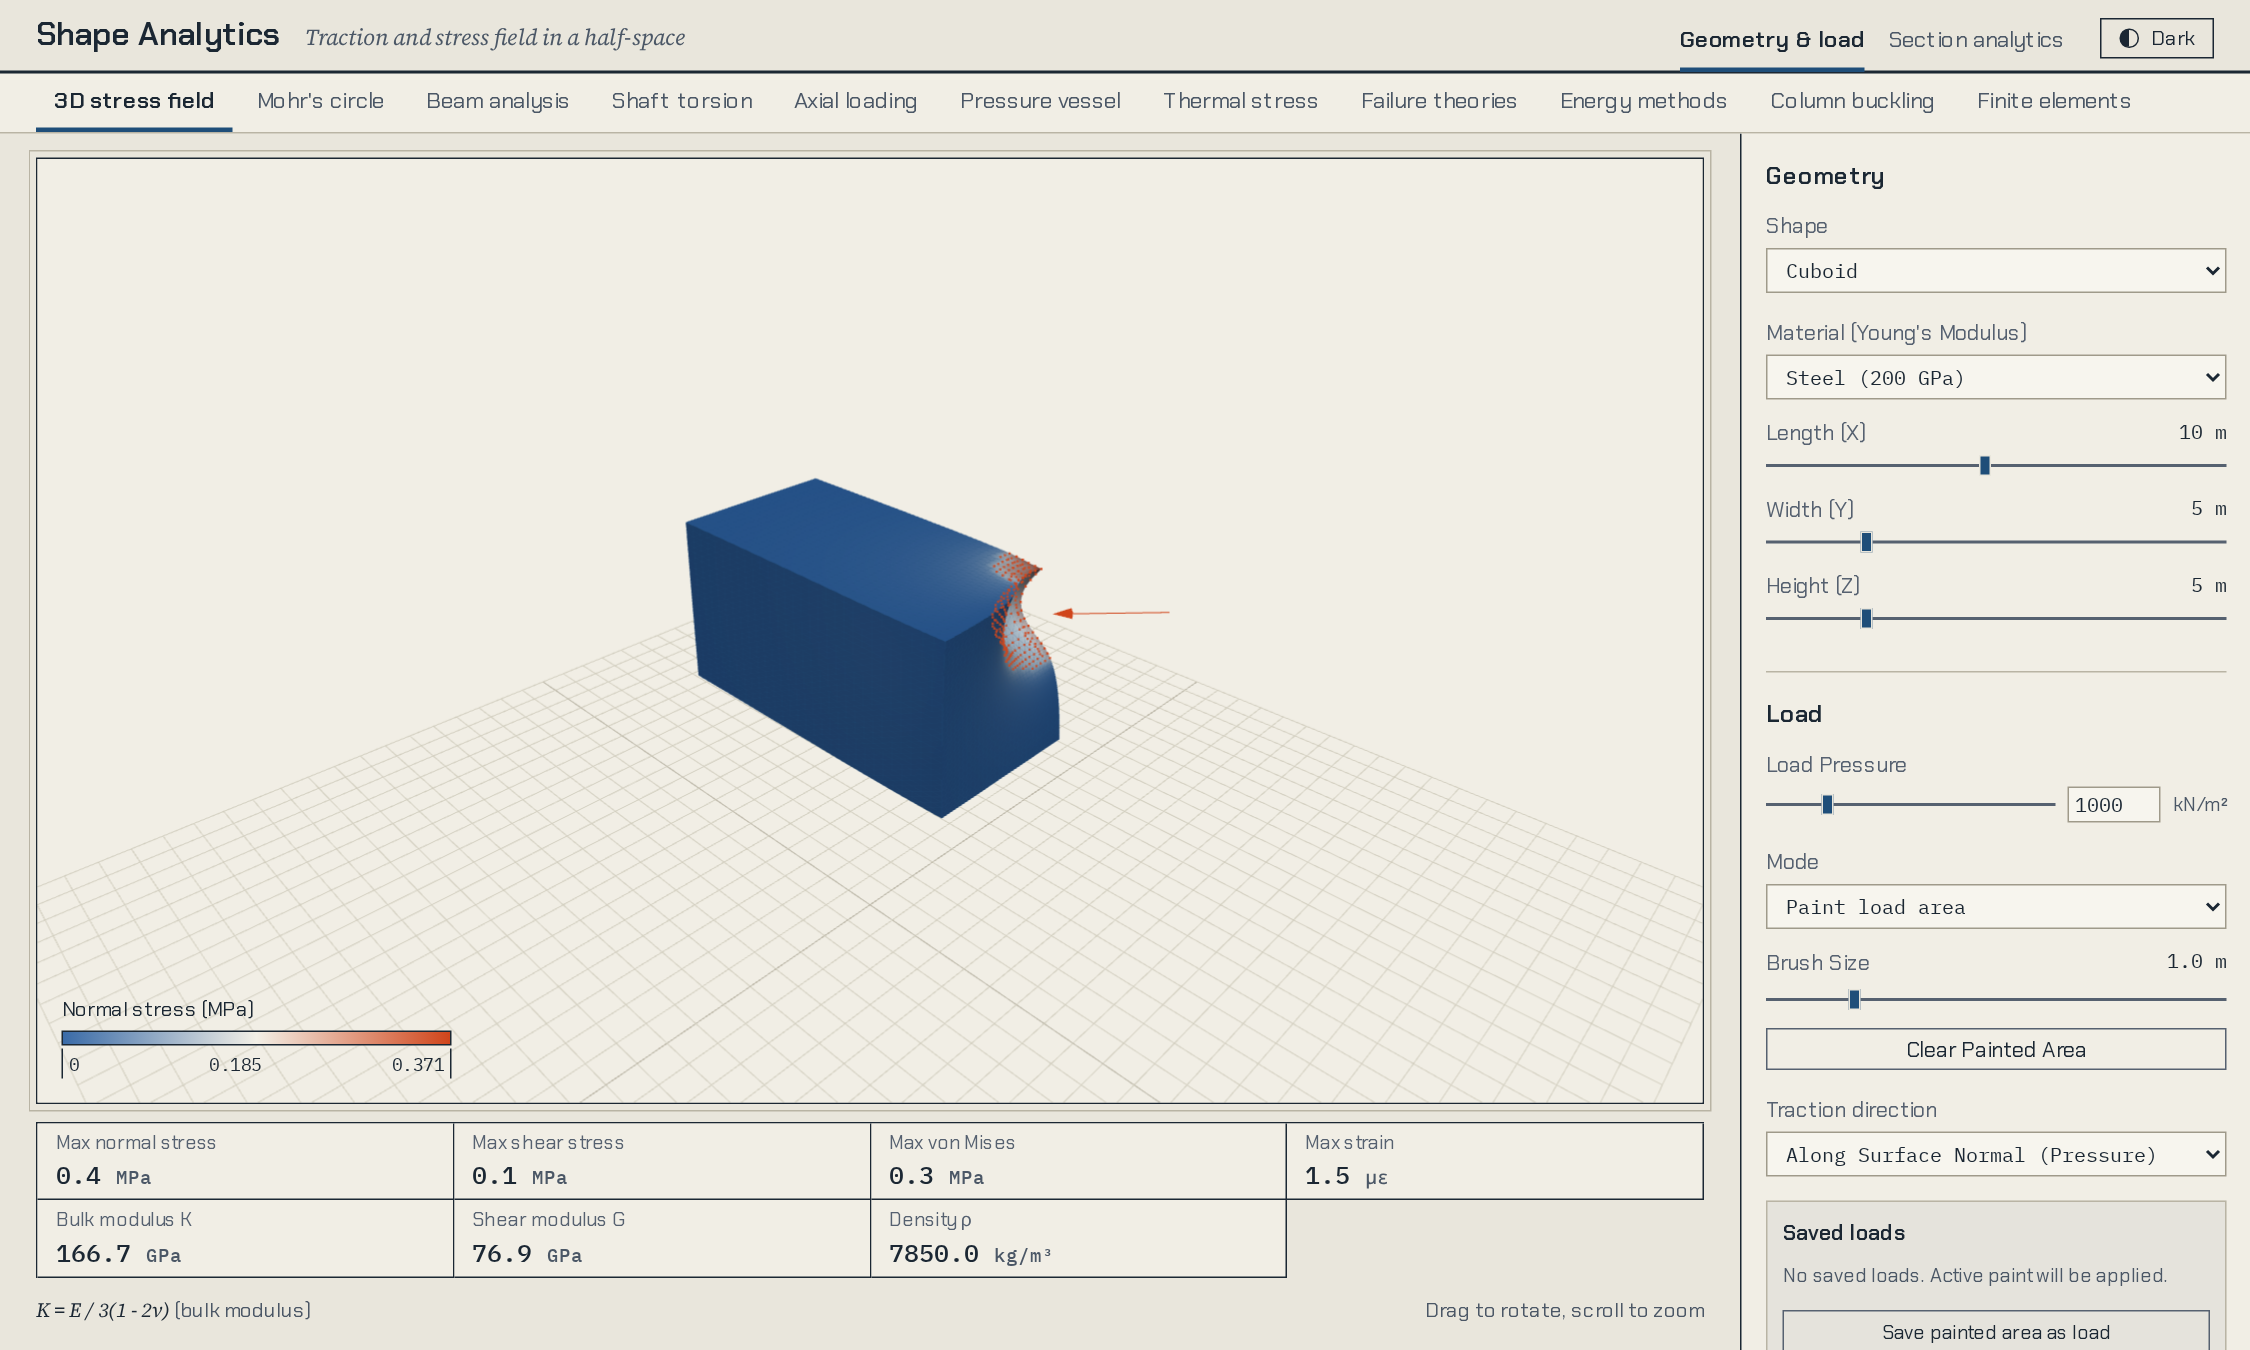
\includegraphics[width=\linewidth]{../figures/ui_field_loaded.png}
\caption{The 3D stress field. A load painted on the top-right edge of a steel cuboid produces the coloured normal-stress map; the navigation bar switches between the nine simulators and the finite element tab. The readout cards below the viewport give the maxima of the displayed measures.}\label{fig:ui-field}
\end{figure}

\section{Conventions and units}
\begin{center}\small
\begin{tabular}{@{}p{3.2cm}p{11.8cm}@{}}\toprule
Sign convention & tension is positive; compressive loads give negative normal stress. In the half-space frames $z$ points \emph{into} the body.\\
Units, 3D field & lengths in metres, forces in newtons, stresses in pascals inside the physics functions, shown as MPa in the interface.\\
Units, simulators & millimetres, newtons, megapascals (so $E$ is in MPa); loads shown in kN, moments in kN\,m.\\
Units, FEM & SI inside the solver; the interface uses mm, kN and MPa.\\
Tensor storage & $[\sigma_{xx},\sigma_{yy},\sigma_{zz},\tau_{xy},\tau_{xz},\tau_{yz}]$ in \texttt{physics.js}; the FEM 3D code orders $[xx,yy,zz,yz,xz,xy]$ (engineering shear strain).\\
Small strain & every model is linear elastic and assumes $|\nabla\mathbf u|\ll1$.\\\bottomrule
\end{tabular}
\end{center}

\section{Source files}
\begin{center}\small
\begin{tabular}{@{}p{3.6cm}p{1.8cm}p{8.9cm}@{}}\toprule
File & Lines & Role\\\midrule
\file{index.html} & 239 & page structure: header, module navigation, the 3D viewport, the analytics drawer, the simulator layout\\
\file{style.css}, \file{fem.css} & 437, 19 & the design tokens, light and dark themes, layouts\\
\file{app.js} & 927 & the 3D field: geometry, painting, loads, the stress computation, the section plots, theme\\
\file{physics.js} & 98 & pure functions for half-space stresses, displacements, principal stresses, von Mises, strain\\
\file{sims.js} & 804 & the nine simulators as configuration objects, plus the framework that renders them\\
\file{fem.js} & 353 & the FEM tab: controls, request, mesh drawing, charts, explanation panels\\
\file{server.py} & 365 & FastAPI app: \texttt{/api/traction}, \texttt{/api/principal}, \texttt{/api/section}, static files\\
\file{fem.py} & 508 & finite element solvers (bar, beam, 2D elements) and the \texttt{/api/fem/solve} route\\
\file{fem3d.py} & 250 & the 3D brick solver and the half-space reference\\
\file{docs/} & --- & this report, \texttt{physics\_report} (physics by chapter), \texttt{fem\_primer}, the FEM plan\\\bottomrule
\end{tabular}
\end{center}

\section{Architecture}
Figure~\ref{fig:arch} shows how the files are connected.
\begin{figure}[!ht]
\centering
\begin{tikzpicture}[x=1cm,y=1cm,font=\footnotesize,
 box/.style={draw=accent,fill=white,rounded corners=1.5pt,align=center,inner sep=4pt,minimum width=2.7cm,minimum height=0.95cm},
 srv/.style={box,fill=paper},
 arr/.style={-{Stealth[length=2mm]},thick,draw=black!75},
 lab/.style={font=\scriptsize,fill=white,inner sep=1.5pt},
 grp/.style={draw=black!45,dashed,rounded corners=3pt,inner sep=7pt}]
\node[box] (html) at (0,0) {\file{index.html}\\layout, tabs};
\node[box] (lib)  at (0,-2.6) {Plotly, Three.js\\(CDN)};
\node[box] (app)  at (4.2,2.6) {\file{app.js}\\3D field};
\node[box] (sims) at (4.2,0) {\file{sims.js}\\9 simulators};
\node[box] (fem)  at (4.2,-2.6) {\file{fem.js}\\FEM tab};
\node[box] (phys) at (8.4,2.6) {\file{physics.js}\\half-space physics};
\node[srv] (srvr) at (12.9,0) {\file{server.py}\\FastAPI};
\node[srv] (femp) at (12.9,-2.6) {\file{fem.py}\\\file{fem3d.py}};
\begin{scope}[on background layer]
\node[grp,fit=(html)(lib)(app)(sims)(fem)(phys)] (browser) {};
\node[grp,fit=(srvr)(femp)] (server) {};
\end{scope}
\node[anchor=south west,font=\scriptsize\bfseries,text=black!60] at (browser.north west) {BROWSER};
\node[anchor=south west,font=\scriptsize\bfseries,text=black!60] at (server.north west) {SERVER};
% index.html loads the three scripts through one trunk, and the libraries
\draw[thick,draw=black!75] (html.east) -- (2.15,0);
\draw[thick,draw=black!75] (2.15,2.6) -- (2.15,-2.6);
\draw[arr] (2.15,2.6) -- (app.west);
\draw[arr] (2.15,0) -- (sims.west);
\draw[arr] (2.15,-2.6) -- (fem.west);
\draw[arr] (html.south) -- node[lab,right=2pt]{loads} (lib.north);
% module registration and physics
\draw[arr] (fem.north) -- node[lab,right=2pt]{registerModule} (sims.south);
\draw[arr] (app.east) -- node[lab,above=1pt,fill=none]{imports} (phys.west);
% API calls
\draw[arr] (app.north) -- ++(0,0.75) -| node[lab,pos=0.25]{POST /api/section} (srvr.north);
\draw[arr] (fem.east) -- node[lab,above=1pt,fill=none]{POST /api/fem/solve} (femp.west);
\draw[arr] (srvr.south) -- node[lab,right=2pt]{mounts router} (femp.north);
\end{tikzpicture}
\caption{Architecture. \file{index.html} loads the scripts and the two libraries; \file{sims.js} and \file{fem.js} register their tabs into one navigation bar. The 3D field is computed in the browser (\file{physics.js}); only the section plots and the FEM solves call the server, which also serves the static files.}\label{fig:arch}
\end{figure}
There is no build step. The three scripts are ES modules loaded by \file{index.html}; \file{sims.js} and \file{fem.js} register themselves into the same navigation bar, so the FEM tab can be removed by deleting its files (see Appendix~\ref{app:ext}). The 3D field computes entirely in the browser; only the section plots (and the FEM solves) are sent to the server, because they need to evaluate thousands of points.

\section{Running the software}
The script \texttt{run\_shape\_analytics.sh} starts \texttt{uvicorn server:app} on port 8002 using the virtual environment of the sibling project. The server mounts the static files, so the page is served from the same origin as the API.

